\documentclass{beamer}
\mode<presentation> {

%\usetheme{default}
\usetheme{Amsterdam}
%\usetheme{AnnArbor}
%\usetheme{Antibes}
%\usetheme{Bergen}
%\usetheme{Berkeley}
%\usetheme{Berlin}
%\usetheme{Boadilla}
%\usetheme{CambridgeUS}
%\usetheme{Copenhagen}
%\usetheme{Darmstadt}
%\usetheme{Dresden}
%\usetheme{Frankfurt}
%\usetheme{Goettingen}
%\usetheme{Hannover}
%\usetheme{Ilmenau}
%\usetheme{JuanLesPins}
%\usetheme{Luebeck}
%\usetheme{Madrid}
%\usetheme{Malmoe}
%\usetheme{Marburg}
%\usetheme{Montpellier}
%\usetheme{PaloAlto}
%\usetheme{Pittsburgh}
%\usetheme{Rochester}
%\usetheme{Singapore}
%\usetheme{Szeged}
%\usetheme{Warsaw}

% As well as themes, the Beamer class has a number of color themes
% for any slide theme. Uncomment each of these in turn to see how it
% changes the colors of your current slide theme.

%\usecolortheme{albatross}
%\usecolortheme{beaver}
%\usecolortheme{beetle}
%\usecolortheme{crane}
%\usecolortheme{dolphin}
%\usecolortheme{dove}
%\usecolortheme{fly}
%\usecolortheme{lily}
%\usecolortheme{orchid}
%\usecolortheme{rose}
%\usecolortheme{seagull}
%\usecolortheme{seahorse}
%\usecolortheme{whale}
%\usecolortheme{wolverine}

%\setbeamertemplate{footline} % To remove the footer line in all slides uncomment this line
%\setbeamertemplate{footline}[page number] % To replace the footer line in all slides with a simple slide count uncomment this line
\setbeamertemplate{navigation symbols}{}
}
\usepackage[utf8]{inputenc}
\usepackage{graphicx} % Allows including images
\usepackage{booktabs} % Allows the use of \toprule, \midrule and \bottomrule in tables
\usepackage{circuitikz}
\usepackage{tikz}
\usetikzlibrary{matrix,calc}
\usetikzlibrary{positioning}



\newcommand{\implicant}[3][0]{
    \draw[rounded corners=3pt] ($(#2.north west)+(135:#1)$) rectangle ($(#3.south east)+(-45:#1)$);
    }

%group lateral borders
%#1-space between node and grouping line. Default=0
%#2-top left node
%#3-bottom right node
\newcommand{\implicantcostats}[3][0]{
    \draw[rounded corners=3pt] ($(rf.east |- #2.north)+(90:#1)$)-| ($(#2.east)+(0:#1)$) |- ($(rf.east |- #3.south)+(-90:#1)$);
    \draw[rounded corners=3pt] ($(cf.west |- #2.north)+(90:#1)$) -| ($(#3.west)+(180:#1)$) |- ($(cf.west |- #3.south)+(-90:#1)$);
}

%group top-bottom borders
%#1-space between node and grouping line. Default=0
%#2-top left node
%#3-bottom right node
\newcommand{\implicantdaltbaix}[3][0]{
    \draw[rounded corners=3pt] ($(cf.south -| #2.west)+(180:#1)$) |- ($(#2.south)+(-90:#1)$) -| ($(cf.south -| #3.east)+(0:#1)$);
    \draw[rounded corners=3pt] ($(rf.north -| #2.west)+(180:#1)$) |- ($(#3.north)+(90:#1)$) -| ($(rf.north -| #3.east)+(0:#1)$);
}

%group corners
%#1-space between node and grouping line. Default=0
\newcommand{\implicantcantons}[1][0]{
    \draw[rounded corners=3pt] ($(rf.east |- 0.south)+(-90:#1)$) -| ($(0.east |- cf.south)+(0:#1)$);
    \draw[rounded corners=3pt] ($(rf.east |- 8.north)+(90:#1)$) -| ($(8.east |- rf.north)+(0:#1)$);
    \draw[rounded corners=3pt] ($(cf.west |- 2.south)+(-90:#1)$) -| ($(2.west |- cf.south)+(180:#1)$);
    \draw[rounded corners=3pt] ($(cf.west |- 10.north)+(90:#1)$) -| ($(10.west |- rf.north)+(180:#1)$);
}
\def\ol#1{\overline{#1}}
%Empty Karnaugh map 4x4
\newenvironment{Karnaugh}%
{
\begin{tikzpicture}[baseline=(current bounding box.north),scale=0.8]
\draw (0,0) grid (4,4);
%
\matrix (mapa) [matrix of nodes,
        column sep={0.8cm,between origins},
        row sep={0.8cm,between origins},
        every node/.style={minimum size=0.3mm},
        anchor=8.center,
        ampersand replacement=\&] at (0.5,0.5)
{
                       \& |(c00)| $\ol{yw}$  \& |(c01)| $\ol{y}w$  \& |(c11)| $yw$       \& |(c10)| $y\ol{w}$  \& |(cf)| \phantom{00} \\
|(r00)| $\ol{xz}$      \& |(0)|  \phantom{0} \& |(1)|  \phantom{0} \& |(3)|  \phantom{0} \& |(2)|  \phantom{0} \&                     \\
|(r01)| $\ol{x}z$      \& |(4)|  \phantom{0} \& |(5)|  \phantom{0} \& |(7)|  \phantom{0} \& |(6)|  \phantom{0} \&                     \\
|(r11)| $xz$           \& |(12)| \phantom{0} \& |(13)| \phantom{0} \& |(15)| \phantom{0} \& |(14)| \phantom{0} \&                     \\
|(r10)| $x\ol{z}$      \& |(8)|  \phantom{0} \& |(9)|  \phantom{0} \& |(11)| \phantom{0} \& |(10)| \phantom{0} \&                     \\
|(rf) | \phantom{00}   \&                    \&                    \&                    \&                    \&                     \\
};
}%
{
\end{tikzpicture}
}

%Empty Karnaugh map 2x4
\newenvironment{Karnaughvuit}%
{
\begin{tikzpicture}[baseline=(current bounding box.north),scale=0.8]
\draw (0,0) grid (4,2);
%
\matrix (mapa) [matrix of nodes,
        column sep={0.8cm,between origins},
        row sep={0.8cm,between origins},
        every node/.style={minimum size=0.3mm},
        anchor=4.center,
        ampersand replacement=\&] at (0.5,0.5)
{
                      \& |(c00)| $\ol{BA}$  \& |(c01)| $\ol{B}A$  \& |(c11)| $BA$       \& |(c10)| $B\ol{A}$  \& |(cf)| \phantom{00} \\
|(r00)| $\ol{C}$      \& |(0)|  \phantom{0} \& |(1)|  \phantom{0} \& |(3)|  \phantom{0} \& |(2)|  \phantom{0} \&                     \\
|(r01)| $C$           \& |(4)|  \phantom{0} \& |(5)|  \phantom{0} \& |(7)|  \phantom{0} \& |(6)|  \phantom{0} \&                     \\
|(rf) | \phantom{00}  \&                    \&                    \&                    \&                    \&                     \\
};
}%
{
\end{tikzpicture}
}

%Defines 8 or 16 values (0,1,X)
\newcommand{\contingut}[1]{%
\foreach \x [count=\xi from 0]  in {#1}
     \path (\xi) node {\x};
}

%Places 1 in listed positions
\newcommand{\minterms}[1]{%
    \foreach \x in {#1}
        \path (\x) node {1};
}

%Places 0 in listed positions
\newcommand{\maxterms}[1]{%
    \foreach \x in {#1}
        \path (\x) node {0};
}

%Places X in listed positions
\newcommand{\indeterminats}[1]{%
    \foreach \x in {#1}
        \path (\x) node {X};
}








%----------------------------------------------------------------------------------------
%	TITULOS
%----------------------------------------------------------------------------------------
\title[Seminario de tecnología]{Unidad I\\ Electrónica analógica}
\author{David A. Trejo Pizzo}
\institute[Instituto Multimedial Da Vinci]
{Departamento de sistemas\\
\medskip
\textit{dtrejopizzo@gmail.com}}
\date{Marzo, 2015}
\begin{document}
\begin{frame}
\titlepage
\end{frame}


%----------------------------------------------------------------------------------------
%	INDICE
%----------------------------------------------------------------------------------------
\begin{frame}
\frametitle{Estructura}
\tableofcontents
\end{frame}


%----------------------------------------------------------------------------------------
%	SLIDES
%----------------------------------------------------------------------------------------

%------------------------------------------------

\section{Introducción}

\begin{frame}
\frametitle{Que es?}

\begin{itemize}
\item 20' - La ciencia que estudia el comportamiento de los electrones en los tubos de vacío.
\item 40' - La ciencia que estudia y aprovecha la electricidad mediante dispositivos semiconductores y otros.
\item 50' - La rama de la ingeniería que estudia el aprovechamiento de la electricidad en diferentes componentes o dispositivos para generar, transmitir o almacenar información, y otras aplicaciones.
\end{itemize}
\end{frame}
%------------------------------------------------

\begin{frame}
\frametitle{Ramas}
\begin{columns}[c]

\column{.5\textwidth}
Electrónica analógica\\

Estudia los sistemas cuyas variables (tensión, corriente, etcétera) varían de una forma continua en el tiempo y pueden tomar (al menos teóricamente) valores infinitos.

\column{.5\textwidth}
Electrónica digital\\

Las variables solo pueden tomar valores discretos y tienen siempre un estado perfectamente definido.

\end{columns}
\end{frame}
%------------------------------------------------

\subsection{Electricidad}
\begin{frame}
\frametitle{Electricidad}

\end{frame}
%------------------------------------------------

\begin{frame}
\frametitle{Cargas eléctricas}

La materia esta formada por átomos, compuestos por protones, neutrones y electrones. Los electrones tienen carga eléctrica negativa y los protones carga positiva. En estado neutro, existen igual número de electrones que de protones. Si se pierde el equilibrio se le llama ion positivo si ha perdido electrones o ion negativo si tiene exceso de electrones. La unidad para medir la carga eléctrica es el Coulomb:
1 Coulomb = $6.28x10^{18}$ electrones.

\begin{figure}[!h]
\centering
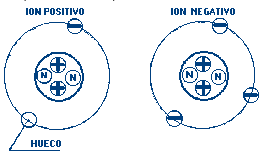
\includegraphics[width=2in]{cargas}
\end{figure}

\end{frame}
%------------------------------------------------

\begin{frame}
\frametitle{Corriente eléctrica}

Si en un espacio físico o un cuerpo hay acumulación de cargas positivas en un sitio y negativas en otro se produce un movimiento de electrones de la zona negativa a la positiva, al movimiento de electrones se llama corriente eléctrica. La corriente eléctrica se indica por una flecha y la letra I sobre el elemento por el que pasa la corriente (obsérvese que la corriente es contraria al movimiento de los electrones). La corriente se mide por la cantidad de carga que pasa en la unidad de tiempo.

Su unidad es el amperio.

\end{frame}
%------------------------------------------------

\section{Electrónica analógica}

\subsection{Análisis en DC}

\begin{frame}
\frametitle{Ley de corrientes de Kirchoff}

La suma algebraica de las corrientes en un nodo es cero. Se considera positiva una corriente que entra al nodo y negativa una corriente que sale del nodo.

$$I_{A} + I_{B} - I_{C} - I_{D} + I_{E} = 0$$

La suma de corrientes que entran a un nodo es igual a la suma de corrientes que salen del nodo.

$$I_{B} + I_{E} = I_{A} + I_{C} + I_{D}$$

\end{frame}
%------------------------------------------------

\begin{frame}
\frametitle{Ley de tensiones de Kirchoff}

La suma de voltajes en una trayectoria cerrada o en una malla de un circuito es igual a cero, para la evaluación numérica se toma como positivo el voltaje si se trata de una elevación de voltaje al pasar por el elemento y negativo si hay una caída de voltaje.

\end{frame}
%------------------------------------------------



\begin{frame}
\frametitle{Estructura de los circuitos}

\begin{itemize}
\item Circuito en serie: dos elementos o circuitos están conectados en serie cuando son los dos únicos elementos que están conectados a un nodo. Como consecuencia de la ley de Corrientes de Kirchhoff las corrientes en dos o más elementos en serie son iguales: $I_{A} = I_{B}$.
\end{itemize}

\begin{figure}[!h]
\centering
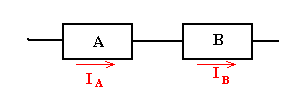
\includegraphics[width=3in]{serie}
\end{figure}

\end{frame}
%------------------------------------------------


\begin{frame}
\frametitle{Estructura de los circuitos}

\begin{itemize}
\item Circuito en paralelo: dos elementos o circuitos están conectados en paralelo cuando los terminales de ambos elementos están conectados a dos nodos comunes. Como consecuencia de la ley de Voltajes de Kirchhoff las tensiones en dos o más elementos en paralelo son iguales: $V_{A} = V_{B}$
\end{itemize}

\begin{figure}[!h]
\centering
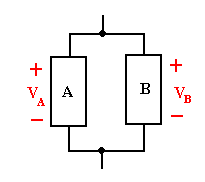
\includegraphics[width=2in]{paralelo}
\end{figure}

\end{frame}
%------------------------------------------------

\begin{frame}
\frametitle{Ley de Ohm}

\begin{figure}[!h]
\centering
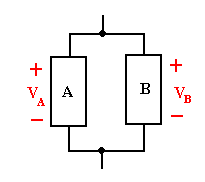
\includegraphics[width=2in]{paralelo}
\end{figure}
\end{frame}
%------------------------------------------------


\begin{frame}
\frametitle{}

\end{frame}
%------------------------------------------------

\subsection{Análisis en AC}

\begin{frame}
\frametitle{}

\end{frame}
%------------------------------------------------

\subsection{Componentes}
\begin{frame}
\frametitle{Componentes activos y pasivos}

\end{frame}
%------------------------------------------------

\subsection{Circuitos integrados}

\begin{frame}
\frametitle{}

\end{frame}
%------------------------------------------------
\end{document}